\documentclass[xcolor={table,usenames,dvipsnames}]{article}
\usepackage{ccicons}
\usepackage[french]{babel}
\setlength{\parindent}{0pt}
\setlength{\parskip}{6pt}  % Adds spacing between paragraphs

\usepackage{caption}
\captionsetup{justification=centering}
\usepackage{tcolorbox} % For the title box
\usepackage{xcolor}    % For colors
\usepackage{graphicx}  % For inserting images
\definecolor{BlueViolet}{RGB}{5, 9, 141} % Define the missing BlueViolet color
\usepackage{hyperref}  % For clickable Table of Contents
 \hypersetup{
	colorlinks=true,      % Enable colored links
	linkcolor=violet,        % Color for internal links (sections, equations, etc.)
	citecolor=BlueViolet,      % Color for citations
	filecolor=magenta,    % Color for file links
	urlcolor=BlueViolet         % Color for URLs
}




\let\oldnocite\nocite
\makeatletter
\renewcommand*{\nocite}[1]{\oldnocite{#1}\Hy@backout{#1}}
\makeatother



\usepackage[style=authoryear, maxbibnames=99, mincitenames=1, maxcitenames=2, backref=true, hyperref=true, dashed=false, firstinits=true, backend=bibtex, bibencoding=utf8, uniquename=false, uniquelist=false, natbib=true]{biblatex}
\renewcommand*{\bibfont}{\scriptsize}

% Remove quotation marks from titles
\DeclareFieldFormat[article,incollection,inproceedings,conference]{title}{#1} 

% Define a custom color for the title box
\definecolor{myblue}{RGB}{44, 62, 80}

\addbibresource{bibliographie.bib} 

\author{Ljudmila PETKOVI\'C}
\title{\textbf{\textsc{M2SOL034} Corpus, ressources et linguistique outillée}}

\begin{document}
	
	% Insert the logo at the top (centered)
	\begin{center}
		
\includegraphics[width=3cm]{img/logo.png} % Adjust width as needed
	\end{center}
	
	% Create a rectangle around the title
	\begin{tcolorbox}[colback=myblue!10, colframe=myblue, width=\textwidth, sharp corners, boxrule=1pt]
		\centering
		\Large \textbf{\textsc{M2SOL034} Corpus, ressources et linguistique outillée\\{\large\textsc{TD 2} : \texttt{TXM I}}}
	\end{tcolorbox}
	
	\begin{center}
		Ljudmila PETKOVI\'C
		
		{\small Sorbonne Université\\Master \og{}Langue et Informatique\fg{} (\textsc{M1} ScLan)\\\textsc{UFR} Sociologie et Informatique pour les Sciences Humaines\\Semestre 2, 2024-2025, le \today}
	\end{center}
	


		
	% Hyperlinked Table of Contents
	\tableofcontents
	
	\bigskip
	
	\section{Exercices : commandes de base}  % Clickable in ToC
	
	\begin{enumerate}
		\item Après avoir installé \texttt{TXM}, chargez\footnote{charger : corpus déjà importé dans \texttt{TXM} auparavant ; importer : corpus brut (\texttt{txt}, \texttt{XML}, voire en provenance du presse-papier).} le corpus \texttt{VOEUX} déjà importé dans \texttt{TXM}, et accédez aux proriétés du corpus. \\
		Indiquez (a) l'année la plus ancienne et (b) l'année la plus récente de l'édition.
		\item Téléchargez le corpus sous format \texttt{XML-TEI} \texttt{charcot.xml} depuis Moodle (\textit{cf.} le répertoire \texttt{ressources\_TD2}), et importez-le dans \texttt{TXM}.\\
		En une seule requête, affichez la liste des mots-pivots dérivés du mot \texttt{hystérie}.
		\item Téléchargez le corpus \textit{Du côté de chez Swann} de Marcel Proust sous format texte brut depuis le site du projet Gutenberg \url{https://www.gutenberg.org/ebooks/2650}, et importez-le dans \texttt{TXM}. Exportez le lexique du corpus importé dans un tableur. Que pouvez-vous constater concernant la répartition des fréquences de mots ?
		\item Trouver en une seule recherche les des mots-pivots dérivés du mot \og{}patrie\fg{} à partir du corpus \texttt{VOEUX}. Quels mots avez-vous extrait ?
		\item Trouver en une seule recherche le souhait de bonne année de chaque Président dans le corpus \texttt{VOEUX}.
		\item Affichez la liste des cooccurrents du terme \texttt{hystérie}, avec leurs fréquences, leurs indices de spécificité et leurs distances moyennes à partir du corpus \texttt{CHARCOT}.\\
		Quel est l'indice de spécificité et la distance moyenne du cooccurrent \texttt{convulsive} ?\\
		Comment interprétez-vous ces mesures ?
		\item Construisez, à l’aide de \texttt{TXM} et sur un tableur un graphique illustrant la loi de Zipf sur le texte de votre choix. Analysez les résultats obtenus.
	
	\end{enumerate}
	
	\bigskip
	
\section{Solutions}
\textit{NB :} les calculs ont été effectués dans la version \textsc{0.8.1} du \texttt{TXM} sur Mac.
\begin{enumerate}
	\item
	\begin{enumerate}
		\item l'année la plus ancienne : 1959 
		\item l'année la plus récente : 2012
 	\end{enumerate}
 	
 	\item Nous obtenons une liste des mots-pivots dérivés du mot \texttt{hystérie} à partir du corpus \texttt{CHARCOT} :
 	\begin{figure}[h] % Use [H] to force the figure to stay in place
 		\centering
 		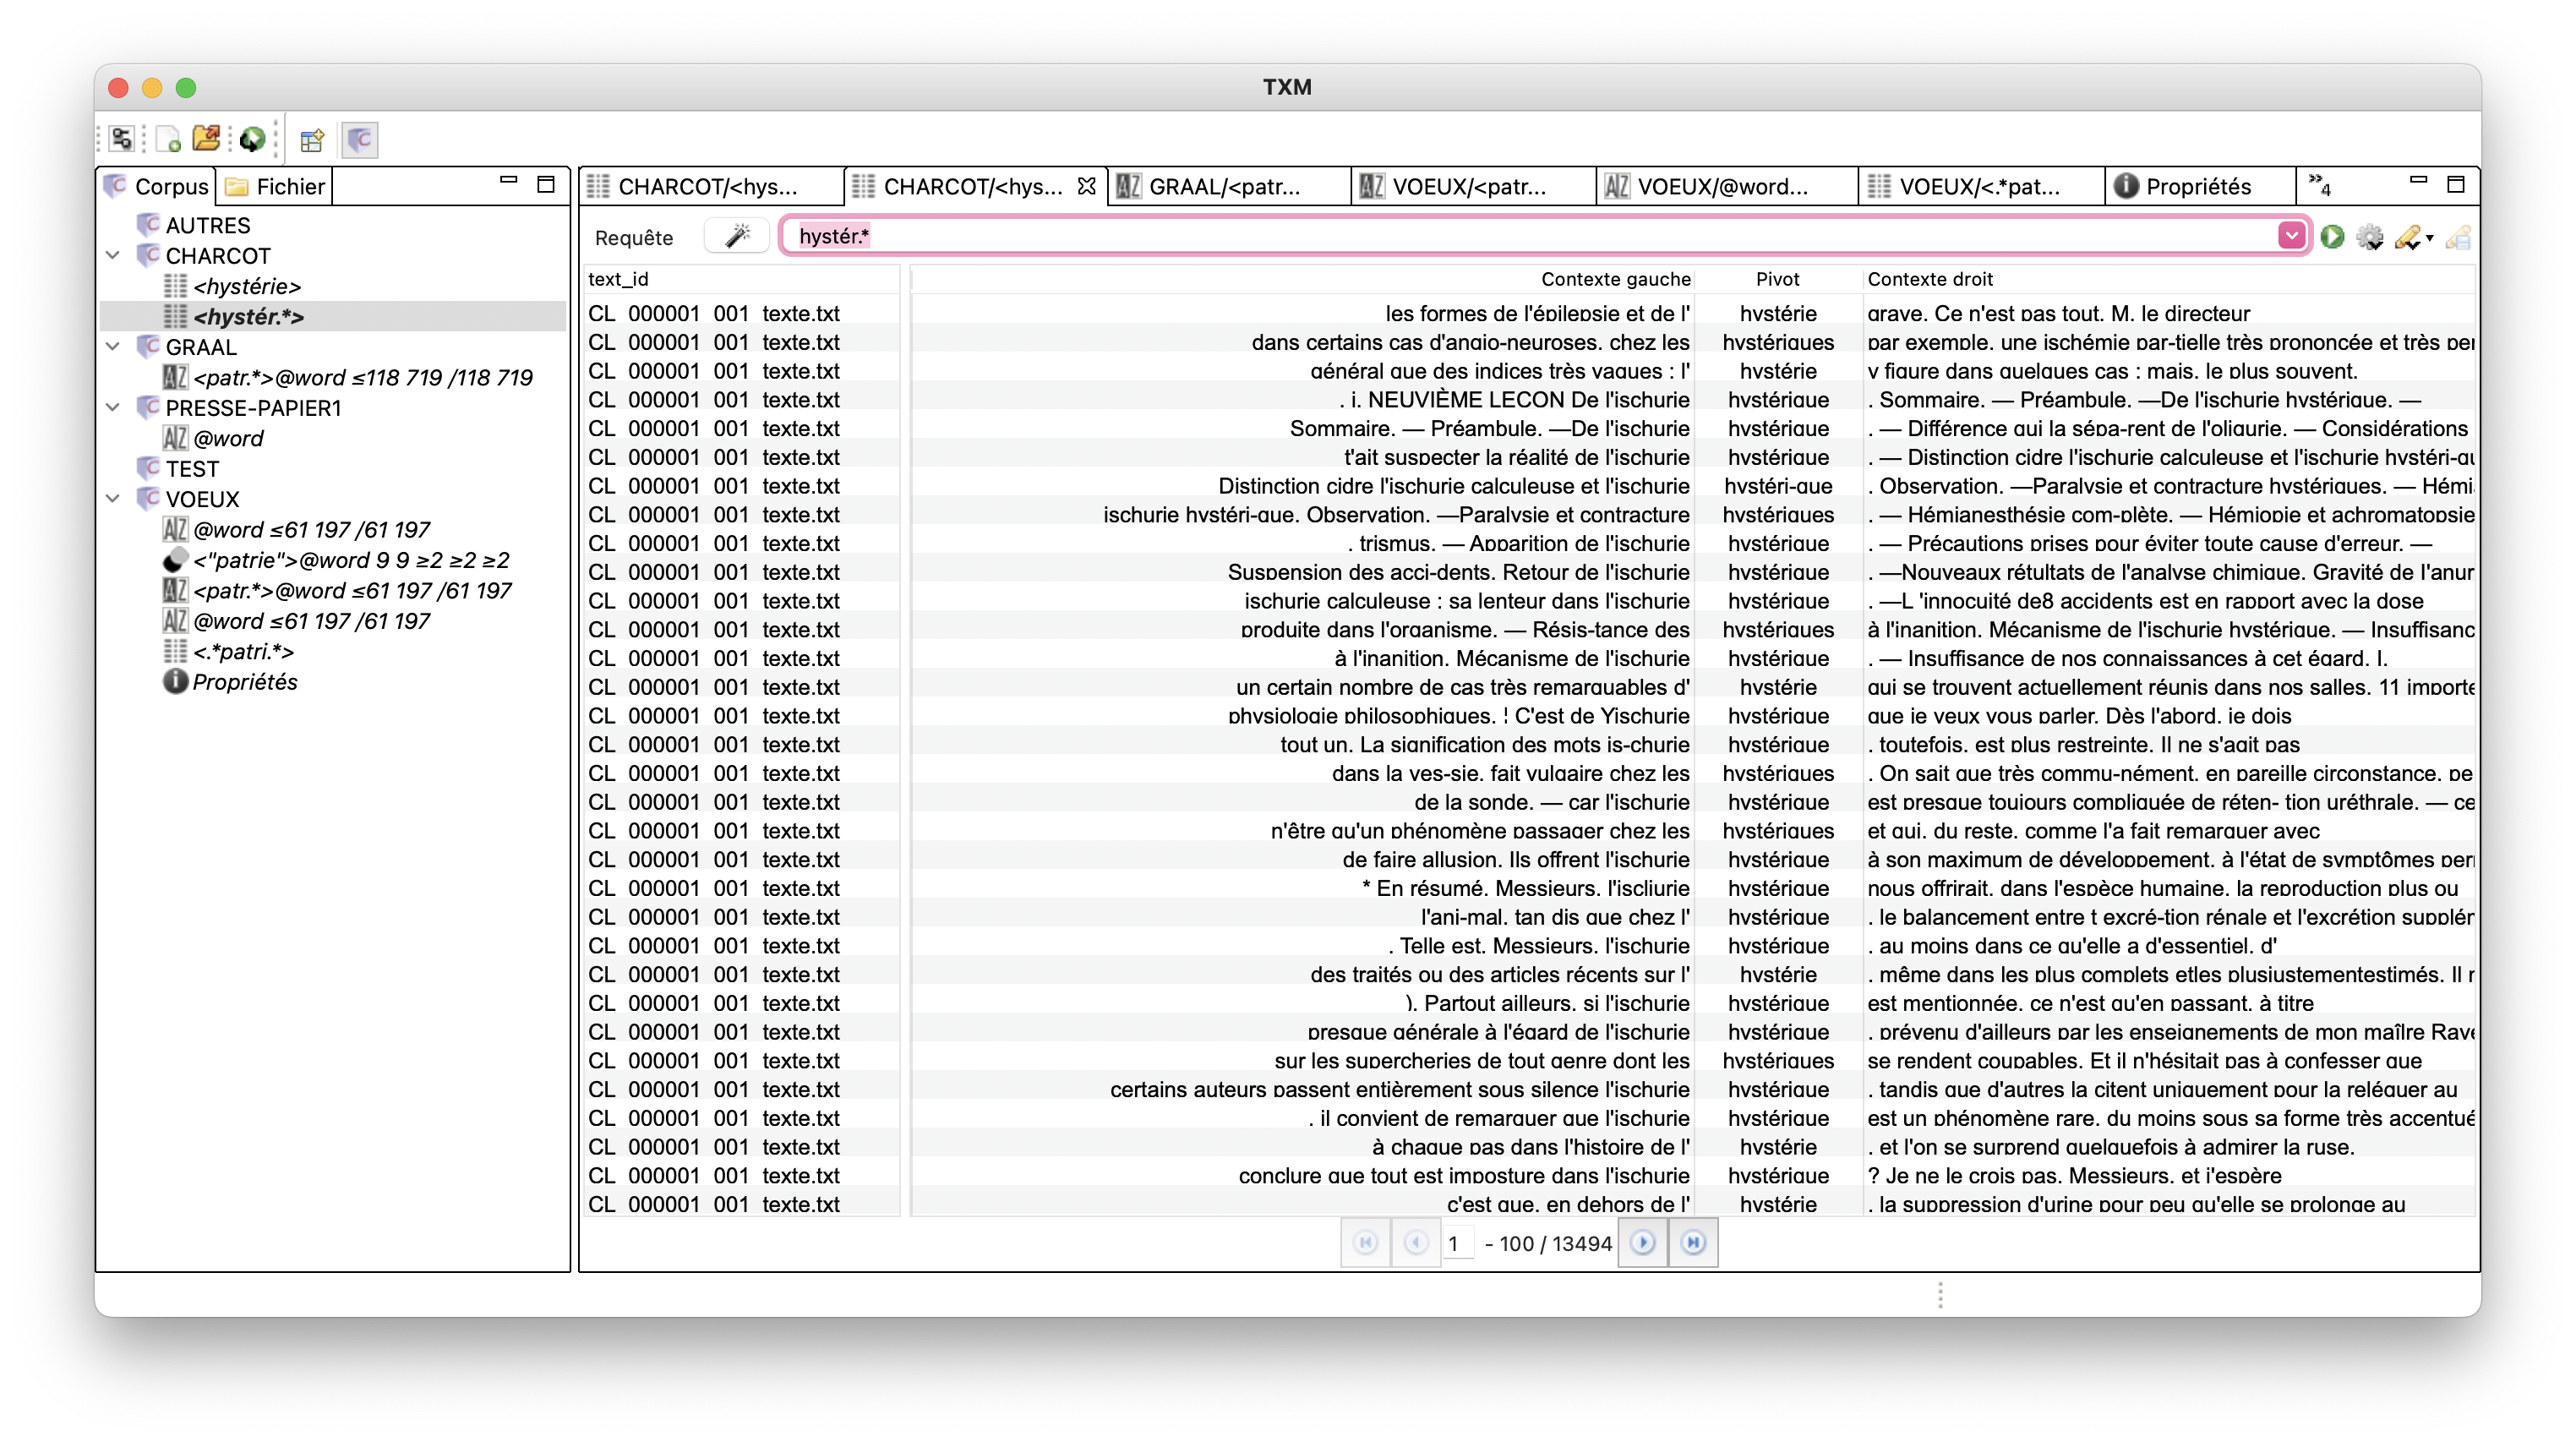
\includegraphics[width=0.80\linewidth]{img/hysterie.png}
 		\label{fig:ling_out_TAL}
 	\end{figure}
 	
 	\item Le lexique du corpus importé montre une distribution des fréquences lexicales évoquant la loi de Zipf, selon laquelle la fréquence d'un mot est inversement proportionnelle à son rang dans la liste globale des mots après le tri par ordre décroissant de fréquence. Autrement dit, peu de mots apparaissent très souvent, tandis que la majorité des mots apparaissent rarement.
 	
 	\item Afin de récupérer les fréquences des mots-pivots dérivés du mot \og{}patrie\fg{}, nous utilisons l'expression régulière \texttt{.*patri.*}. Cela nous permet d'extraire les mots \textit{patrie}, \textit{patriote}, \textit{patriotisme}, \textit{compatriotes} et \textit{rapatriés}.
 	
 	\item \texttt{[frlemma="je"][]*[frlemma="souhaiter"][]*[frlemma="année"] within s}
 	\item L'indice de spécificité du cooccurrent \texttt{convulsive} est \textsc{9} et la distance moyenne est \textsc{1.3}.\\ Concernant l'indice de spécificité, plus il est élevé, plus
 	la cooccurrence est remarquable. \\
 	Pour ce qui est de la distance moyenne, elle indique le nombre de mots entre le cooccurrent et le pivot quand ils sont dans le même voisinage.
 	\item Discussion en \textsc{TD}.
 	
\end{enumerate}


\hrulefill

		\printbibliography
		
		
	\centering
{\small Le contenu de cette présentation est sous licence \texttt{CC-BY-NC-SA 4.0}\\Utilisation non commerciale -- Partage dans les mêmes conditions.\\}
\href{https://creativecommons.org/licenses/by-nc-sa/4.0/deed.fr}{\ccbyncsa}
	
\end{document}
